\documentclass[10pt, a4paper]{article} % 设置字体大小和纸张类型
\usepackage{ctex}
\usepackage{caption} % 插图和表格的标题格式
\usepackage{amsmath, amsfonts, amssymb} % 数学公式支持
\usepackage{graphicx} % 插入图片
\usepackage{hyperref} % 超链接支持
\usepackage{geometry}
\usepackage{titlesec}
\usepackage{fmtcount} % 用于数字到中文的转换
\usepackage{enumitem} % 加载 enumitem 宏包
\geometry{a4paper, margin=1.5cm} % 设置页边距

\renewcommand{\thesection}{\chinese{section}、}
\renewcommand{\thesubsection}{\arabic{subsection}.}


\begin{document}

\begin{titlepage}
    \newgeometry{left=0cm, right=0cm, top=0cm, bottom=0cm}
    \centering
    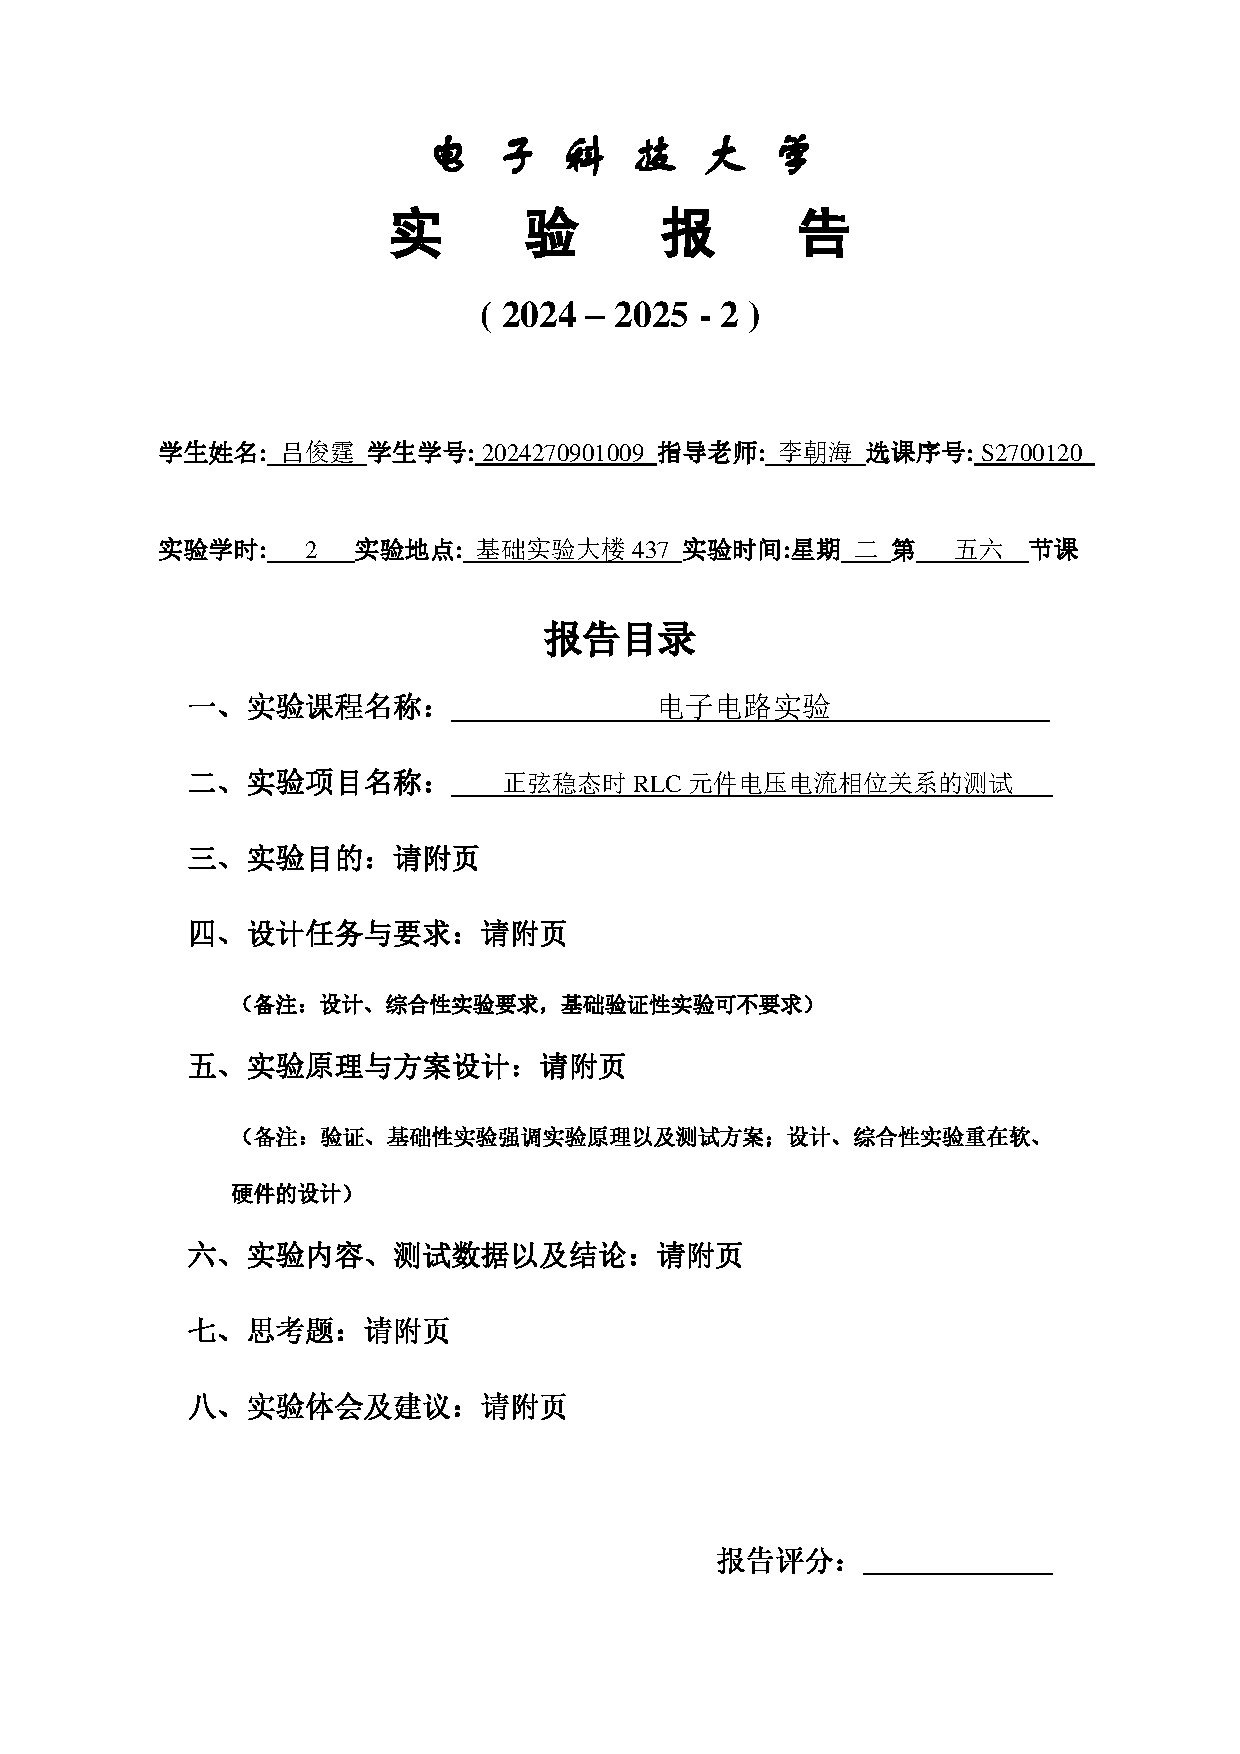
\includegraphics[page=1, width=0.9\textwidth, keepaspectratio]{image/实验报告撰写封面.pdf}
    \restoregeometry
\end{titlepage}

\setcounter{section}{2}

\section{实验目的}

\begin{enumerate}[leftmargin=50pt,label=(\arabic*)] % 设置序号格式为(1)
    \item 理解正弦稳态电路中R、L、C元件的电压电流关系; 
    \item 掌握截距法测试相位差的方法; 
    \item 进一步熟悉示波器、函数发生器的使用。
\end{enumerate}

\section{设计任务与要求}

\begin{enumerate}[leftmargin=50pt,label=(\arabic*)] % 设置序号格式为(1)
    \item 预习电容、电感元件的电压电流关系方程。试分析正弦激励下、电路稳态时,加在电阻、电容以及电感元件两端的电压与流过元件的电流之间的相位关系。
    \item 预习利用面包板搭建电路
    \item 预习电阻器、电容器和电感器简介
\end{enumerate}

\section{实验原理与方案设计}
\subsection{实验原理}
(1) 电阻上电压电流的相位关系
\vspace{0.5cm}

当电阻工作在正弦稳态时, 在关联参考方向下, 电阻上电压电流关系为
$$
v_R(t) = R \cdot i_{R}(t) = R \cdot I_{Rm} \cdot \cos(\omega t + \varphi_{R})
$$

从上式可以看出, 电阻电压、电流同相, 即电压电流的相位差为零。
\vspace{0.5cm}

(2) 电感上电压电流的相位关系
\vspace{0.5cm}

在关联参考方向下, 电感的电压电流关系为
$$
v_L(t) = L \cdot \frac{di_{L}(t)}{dt}
$$

若流过电感的电流为正弦信号$i_{L}(t) = I_{Lm} \cdot \cos(\omega t + \varphi_{L})$, 则电感上的电压为
$$
v_L(t) = -\omega L \cdot I_{Lm} \cdot \sin(\omega t + \varphi_{L}) = \omega L \cdot I_{Lm} \cdot \cos(\omega t + \varphi_{L} + 90^{\circ})
$$

从上式可以看出, 电感上电压领先于电流$90^{\circ}$。
\vspace{0.5cm}

(3) 电容上电压电流的相位关系
\vspace{0.5cm}

在关联参考方向下, 电容的电压电流关系为
$$
i_{C}(t) = C \cdot \frac{dv_{C}(t)}{dt}
$$
若电容两端的电压为正弦信号$v_{C}(t) = V_{Cm} \cdot \cos(\omega t + \varphi_{C})$, 则电容上的电压为
$$
i_{C}(t) = -\omega C \cdot V_{Cm} \cdot \sin(\omega t + \varphi_{C}) = \omega C \cdot V_{Cm} \cdot \cos(\omega t + \varphi_{C} + 90^{\circ})
$$

从上式可以看出, 电容上电压比电流之后$90^{\circ}$。
\newpage
\subsection{方案设计}
(1) 电压电流相位关系的测试方法

\begin{figure}[ht]
\centering
\begin{minipage}[ht]{0.5\textwidth} % 文字部分占 60% 的宽度
    示波器的电压探头无法直接测量流过R、L、C元件的电流。可以采用间接测量的方法, 即在测试电路中将R/L/C同一个电流取样电阻串联, 通过取样电阻的电压来间接测量流过R/L/C元件的电流。
\end{minipage}%
\hfill % 添加一些水平间距
\begin{minipage}[ht]{0.45\textwidth} % 图片部分占 35% 的宽度
    \centering
    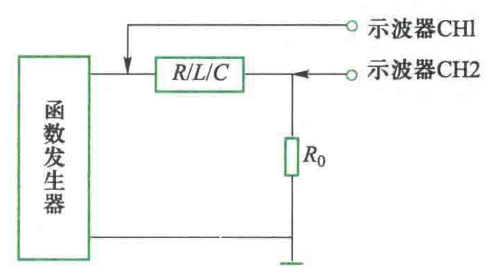
\includegraphics[width=\linewidth]{image/1.png} % 图片宽度占满 minipage
    \captionsetup{font={small}} % 设置图注的字体大小
    \caption{电压电流相位关系的测试原理图}
    \label{fig:side:a}
\end{minipage}
\end{figure}


(2) 同频率两个正弦波形相位差的测量(截距法)
\begin{figure}[ht]
    \centering
    \begin{minipage}[ht]{0.6\textwidth} % 文字部分占 60% 的宽度
        先将示波器的两个通道的零基线与屏幕中间的刻度线调重合, 双踪显示两个电压\(v_1\)和\(v_2\), 如图2所示。从图中可以测量出波形的周期为T, 两个波形的相位差为\(\Delta T\), 一个周期对应的角度为\(360^{\circ}\), 则相位差\(\Delta \varphi\)为
        $$
        \Delta \varphi = \frac{\Delta t}{T} \times 360^{\circ}
        $$
        
        其中, T是一个周期在水平通道所占的格数X与时间因数的乘积, \(\Delta T\)是二者之间的个数$\delta X$与时间因数的乘积, 因此上式可以简化成
        $$
        \Delta \varphi = \frac{\Delta X}{X} \times 360^{\circ}
        $$
    \end{minipage}%
    \hfill % 添加一些水平间距
    \begin{minipage}[ht]{0.35\textwidth} % 图片部分占 35% 的宽度
        \centering
        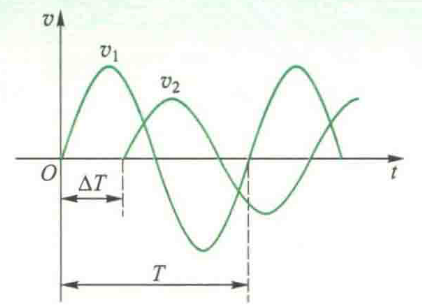
\includegraphics[width=\linewidth]{image/2.png} % 图片宽度占满 minipage
        \captionsetup{font={small}} % 设置图注的字体大小
        \caption{相位差的测量}
        \label{fig:side:b}
    \end{minipage}
    \end{figure}

示波器是从左向右扫描显示的, 因此在图2所示的额波形中, 上升过程中, 电压\(v_1\)先于电压\(v_2\)出现波峰, 所以电压\(v_1\)领先于电压\(v_2\), 或者说电压\(v_2\)滞后于电压\(v_1\)。

\section{实验内容、测试数据以及结论}
实验数据如下图所示:
\begin{figure}[ht]
    \centering
    \begin{minipage}[ht]{0.3\textwidth}
        \centering
        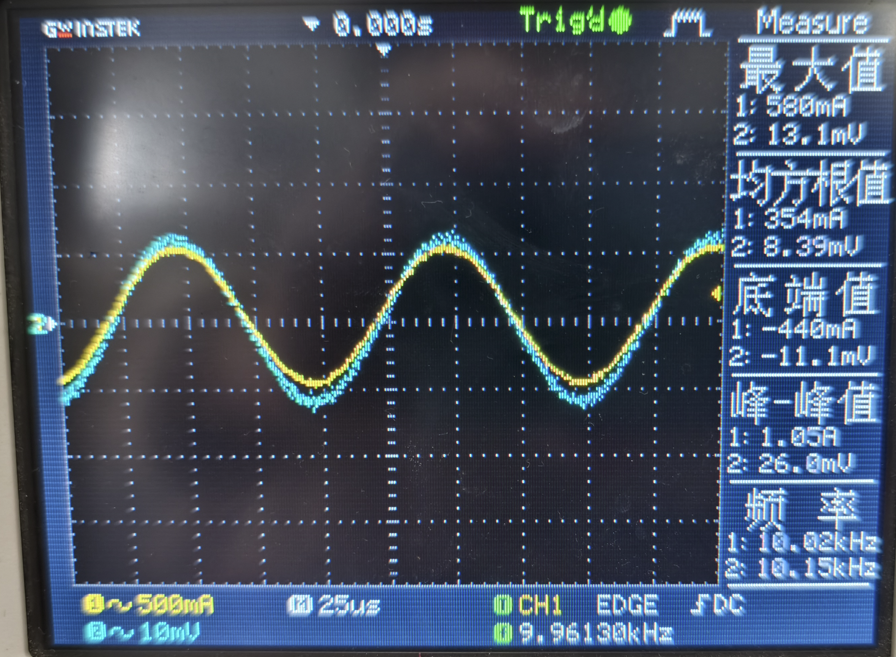
\includegraphics[width=\linewidth]{image/3.png}
        \caption{电阻}
        \label{fig:side:c}
    \end{minipage}
    \hfill
    \begin{minipage}[ht]{0.3\textwidth}
        \centering
        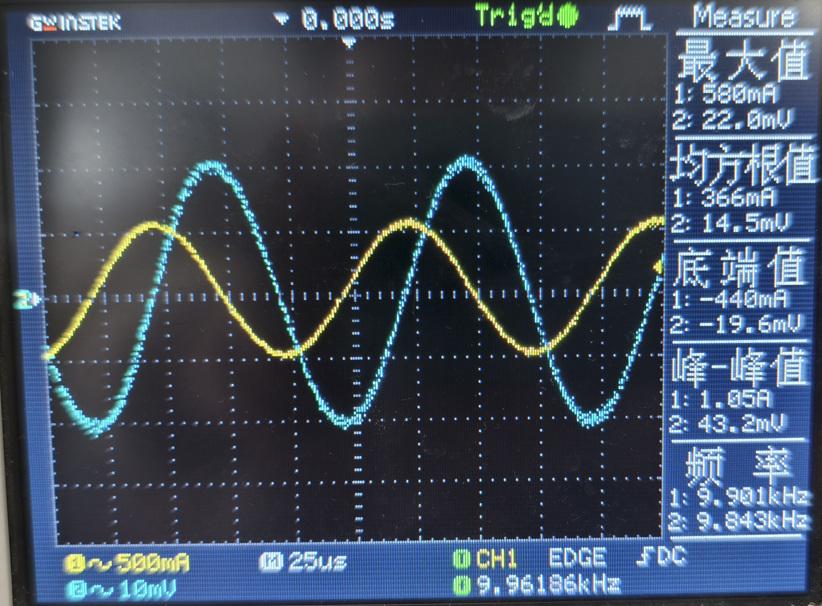
\includegraphics[width=\linewidth]{image/4.png}
        \caption{电感}
        \label{fig:side:d}
    \end{minipage}
    \hfill
    \begin{minipage}[ht]{0.3\textwidth}
        \centering
        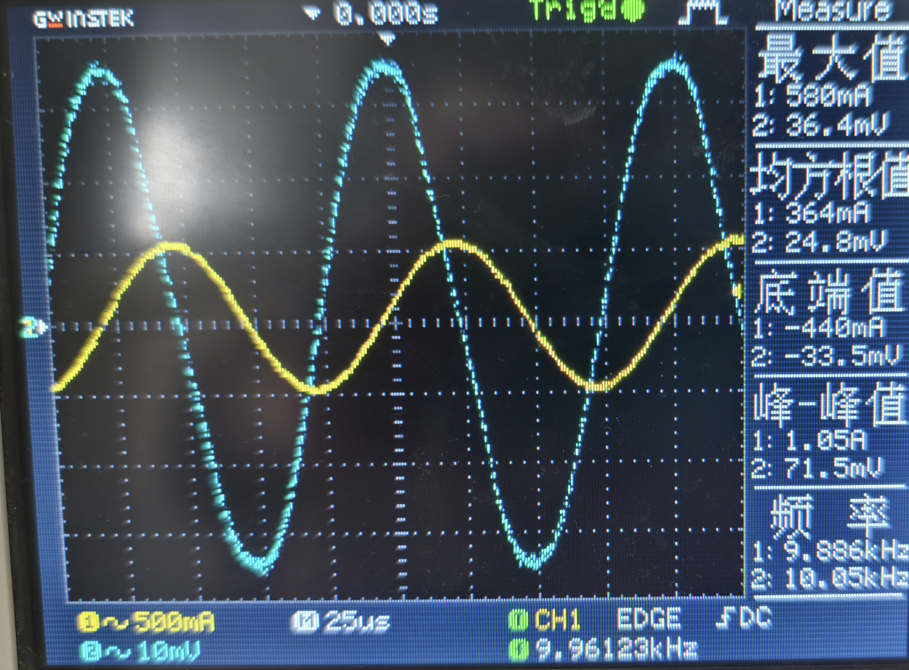
\includegraphics[width=\linewidth]{image/5.png}
        \caption{电容}
        \label{fig:side:e}
    \end{minipage}
\end{figure}

\newpage

\section{思考题}
\subsection{题面}
\begin{enumerate}[leftmargin=50pt,label=(\arabic*)] % 设置序号格式为(1)
    \item 测量相位差时如果示波器两个通道的零基线没有重合, 测出来的相位差正确吗? 此时如何测量才能得到正确结果?
    \item 测量相位差时, 如果改变水平时间因数旋钮或垂直灵敏度旋钮, 会影响测量的结果吗?
\end{enumerate}
\subsection{回答}

\begin{enumerate}[leftmargin=50pt,label=(\arabic*)] % 设置序号格式为(1)
    \item 不正确, 应该调整示波器两个通道的零基线使其重合, 然后再测量相位差。
    \item 会影响, 因为改变水平时间因数旋钮或垂直灵敏度旋钮会改变示波器的显示范围, 从而影响测量的结果。
\end{enumerate}

\section{实验体会及建议}
\subsection{实验体会}
通过本次实验, 我学会了如何测试电阻、电感、电容的电压电流相位关系, 了解了截距法测试相位差的方法, 进一步熟悉了示波器、函数发生器的使用。
\subsection{建议}
应该多注意负载的影响, 保证实验数据的准确性。


\end{document}
